% % % % % % % % % % % % % % 
% 
% Skript zu NUMERIK I
% WS14/15
% von Prof. Dr. Blank
% Universität Regensburg
% 
% 
%	Kap. 3: Fehleranalyse
% 
% % % % % % % % % % % % % % 


\chapter{Fehleranalyse} \index{Fehler}\label{3}
\marginpar{15.10.2014}
\begin{align*}
  \overset{
  x+\varepsilon \text{ statt } x}%
  {\framebox[3cm]{Eingabe}
  } 
  \longrightarrow 
  \overset{
  \underset{\text{\tiny (z.B. durch Rundung)}}{\widetilde{f} \text{ statt } f}}%
  {\framebox[3cm]{Algorithmus}
  } 
  \longrightarrow
  \overset{
  \widetilde{f}(x+\varepsilon) \text{ statt } f(x)}%
  {\framebox[3cm]{Resultat\phantom{g}}
  }
\end{align*}

Bei der Fehleranalyse liegt das Hauptaugenmerk auf
\begin{itemize}
\item[] \textbf{Eingabefehler}\\ z.B.Rundungsfehler, Fehler in Messdaten, Fehler im Modell (falsche Parameter)
\item[] \textbf{Fehler im Algorithmus} \\ z.B. Rundungsfehler durch Rechenoperationen, Approximationen \\
  (z.B. Ableitung durch Differenzenquotient oder die Berechnung von Sinus durch abgebrochene Reihenentwicklung)

\item[\textit{1. Frage}] Wie wirken sich Eingabefehler auf das Resultat unabhängig vom gewählten Algorithmus aus?
\item[\textit{2. Frage}]Wie wirken sich (Rundungs-)Fehler des Algorithmus aus?\\
  Und wie verstärkt der Algorithmus Eingabefehler?
\end{itemize}


\sectione{Zahlendarstellung und Rundungsfehler} \label{3.1} \index{Fehler} \index{Rundungsfehler}\index{Zahlendarstellung}
Auf (Digital-)Rechnern können nur endlich viele Zahlen realisiert werden.
Die wichtigsten Typen sind: 
\begin{itemize}
\item \textbf{ganze Zahlen}  (integer)\index{integer}:
  \begin{align*}
    z&=\pm \sum_{i=0}^{m}z_i\beta_i 
    & \text{mit }
      \begin{array}{l@{\,}l}
        \beta &= \text{Basis des Zahlensystems (oft $\beta=2$)} \\
        z_i &\in \{0, \cdots \beta-1\}
      \end{array}
  \end{align*}
\item \textbf{Gleitpunktzahlen} (floating point) \index{floating point}
\end{itemize}

\begin{Defe}
  \label{3.1.1} \index{Gleitkommazahl}
  Eine Zahl $x\in\Q$ mit einer Darstellung
  \begin{align*}
    x&=\sigma \cdot(a_1 . a_2 \cdots a_t)_{\beta}\cdot \beta^e 
       = \sigma\beta^e \cdot \sum_{\nu=1}^{t}a_\nu \beta^{-\nu+1}\\\\
     &\quad\begin{array}{ll}
             \beta\in\N & \text{Basis des Zahlensystems}\index{Basis}\\
             \sigma \in\{\pm 1\} &\text{Vorzeichen} \\
             m = (a_1 . a_2 \cdots a_t)_{\beta} &\text{Mantisse}\index{Mantisse}\\
             \phantom{m}= \sum_{\nu=1}^{t}a_\nu \beta^{-\nu+1} \\
             a_i \in\{0,\cdots , \beta-1\}&\text{Ziffern der Mantisse}\\
             t\in\N&\text{Mantissenlänge} \\
             e\in\Z &\text{mit }e_{min}\leq e \leq e_{max} \text{ Exponent}
           \end{array}
  \end{align*}
  heißt \textbf{Gleitkommazahl} mit $t$ Stellen und Exponent $e$ zur Basis $b$. \\
  Ist $a_1\neq 0$, so heißt $x$ \textbf{normalisierte Gleitkommazahl}\index{normalisierte Gleitkommazahl}.
\end{Defe}

\begin{Beme}
  \label{3.1.2}~
  \begin{enumerate}[a)]
  \item 0 ist keine normalisierte Gleitkommazahl, da $a_1 =  0$ ist.
  \item $a_1\neq 0$ stellt sicher, dass die Gleitkommadarstellung eindeutig ist.
  \item In der Praxis werden auch nicht-normalisierte Darstellungen verwendet.
  \item Heutige Rechner verwenden meist $\beta =2$, aber auch $\beta=8, \beta=16$.
  \end{enumerate}
\end{Beme}

\subsectione{Bit-Darstellung zur Basis 2}
\label{3.1.3}
Bit-Darstellung nach IEEE-Standard 754 von floating point numbers \\
Sei die Basis $\beta=2$.

\begin{tabular}{l@{}cccc@{}}
  & Speicherplatz & $t$ & $e_{min}$ & $e_{max}$ \\
  \cmidrule{2-5}
  einfache Genauigkeit (float) \index{floating point} & 32bits = 4Bytes & 24 &-126 & 127 \\
  doppelte  Genauigkeit (double)~~\index{double} & 64bits = 8Bytes& 52 & -1022 & 1023
\end{tabular}\\

Darstellung im Rechner (Bitmuster) für float:
\begin{gather*}
  \floatbox{s}{b_0\cdots b_7}{a_2\cdots\cdots a_{24}}\\
  \text{(Da $a_1\neq 0$, also $a_1=1$ gilt, wird $a_1$ nicht gespeichert)}
\end{gather*}

Interpretation ($s,b,a_i\in\{0,1\} \forall i$)
\begin{itemize}
\item $s$ Vorzeichenbit: 
  $\quad \sigma=(-1)^s\Rightarrow 
  \begin{array}{l}
    \sigma(0)=1 \\
    \sigma(1)=-1
  \end{array} $
\item $b=\sum_{i=0}^{7}b_i\cdot2^i \in \{1, \cdots, 254\}$ 
  speichert den Exponenten mit 
  $e = b-\underbrace{127}_{\mathclap{\text{Basiswert}}}$ (kein Vorzeichen nötig).
  Beachte: $b_0=\dotso=b_7=1$ sowie $b_0=\dotso=b_7=0$ sind bis auf Ausnahmen keine gültigen Exponenten
\item $m=(a_1.a_2\dotso a_{24})=1+\sum_{\nu=2}^{24}a_{\nu}2^{1-\nu}$ stellt die Mantisse dar, $a_1=1$ wird nicht abgespeichert.
\item Besondere Zahlen per Konvention:
  \begin{itemize}
  \item[$x=0$:] $s$ bel., $b=0$, $m=1 \quad \floatbox{s}{0\dotso0}{0\dotso0}$
  \item[$x=\pm\infty$:]  $s$ bel., $b=255$, $m=1  \quad \floatbox{s}{1\dots1o}{0\dotso0}$
  \item[$x=$NaN] $s$ bel., $b=255$, $m\neq 1$
  \item[$x=(-1)^s$] $s$ bel., $b=0$, $m\neq 1$ und x hat die Form $x=(0+\sum_{\nu=2}^{24}a_{\nu}\cdot 2^{1-\nu})\cdot 2^{126}$ (\enquote{denormalized} number)
  \end{itemize}
\end{itemize}

% --------------------------------------------------------------------

\marginpar{20.10.2014}
\begin{align*}
  \intertext{Betragsmäßig \textbf{größte Zahl}:}
  \floatbox{0}{01\dotso 1}{ 1\dotso 1} 
  && x_{max} = (2-2^{-23})\cdot 2^{127}  
  & \approx 3,4 \cdot 10^{38}
    \intertext{Betragsmäßig \textbf{kleinste Zahl}:}
    \floatbox{0}{0\dotso 0}{ 0\dotso 01} 
  && x_{min} = 2^{-23}\cdot 2^{-126} = 2^{-149}  
  & \approx 1,4 \cdot 10^{-45}
\end{align*}

\subsectione{Verteilung der Maschinenzahlen} \label{3.1.4}
Die Maschinenzahlen sind ungleichmäßig im Dezimalsystem verteilt, z. B.
\begin{align*}
  x &= \pm a_1 . a_2 a_3 \cdot 2^e  
  &\text{mit } -2\leq e\leq 1 \text{ und } a_i  \in \{0,1\} 
\end{align*}
\begin{image}{\copyright}
  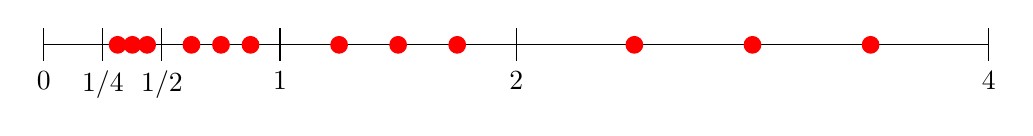
\begin{tikzpicture}[scale=3]
    \draw(0,0)--(4,0);
    % Vertikale Striche
    \foreach \x/\xtext in {0/0,0.25/{1/4},0.5/{1/2},1/1,2/2,4/4}
    \draw(\x,2pt)--(\x,-2pt) node[below] {\xtext};
    % Rote Kreise zeichnen
    \foreach \x in {0.3125,0.375,0.4375,0.625,0.75,0.875,1.25,1.5,1.75,2.5,3,3.5}
    \draw[fill,red] (\x,0) circle (1pt);
  \end{tikzpicture}
\end{image}
ist im Dualsystem gleichmäßig, jedoch im Dezimalsystem sehr ungleichmäßig verteilt.

\begin{Defe}
  \label{3.1.5}~
  \begin{description}
  \item[\textbf{overflow}:] Es ergibt sich eine Zahl, die betragsmäßig größer ist als die größte maschinendarstellbare Zahl.
  \item[\textbf{underflow}:] Entsprechend, betragsmäßig kleiner als die kleinste positive Zahl.
  \end{description}
  Bsp.: overflow beim integer $b=e+127$
  \begin{align*}
    \begin{array}{rrr@{}}
      b &= 254  &11111110 \\
        &+  \phantom{24}3 &00000011 \\
      \cline{3-3} %
      b+3 = 257 \text{ mod } 2^8  &=\phantom{24}1& \xout{1}00000001 
    \end{array}
  \end{align*}
\end{Defe}

\subsectione{Rundungsfehler} \label{3.1.6}
Habe $x\in \R $ die normalisierte Darstellung
\begin{align*}
  x &= \sigma \cdot \beta^e (\sum_{\nu=1}^{t}a_{\nu}\beta^{1-\nu} + \sum_{\nu=t+1}^{\infty}a_{\nu}\beta^{1-\nu} ) \\
    &= \sigma \cdot \beta^e (\sum_{\nu=1}^{t}a_{\nu}\beta^{1-\nu} + \beta^{1-t}\sum_{l=1}^{\infty}a_{t+l}\beta^{-l} )
\end{align*}
mit $e_{min} \leq e \leq e_{max}$, dann wird mit $fl(x)$ die gerundete Zahl bezeichnet, wobei $fl(x)$ 
eindeutig gegeben ist durch die Schranke an den \textbf{absoluten Rundungsfehler} \index{Fehler!absoluter Rundungsfehler}
\begin{align*}
  | fl(x) - x | \leq \begin{cases}
    \frac{1}{2}\beta^{e+1+t} & \text{bei symmetrischem Runden}\\
    \beta^{e+1+t}            & \text{bei Abschneiden}
  \end{cases} \quad .
\end{align*}
Für die \textbf{relative Rechengenauigkeit} \index{Fehler!relative Rechengenauigkeit}folgt somit 
\begin{align*}
  \frac{| fl(x) - x | }{|x|} 
  & \leq 
    \begin{cases}
      \frac{1}{2}\beta^{1-t} & \text{bei symmetrischem Runden}\\
      \beta^{1-t}            & \text{bei Abschneiden}
    \end{cases} \quad .
\end{align*}
Die \textbf{Maschinengenauigkeit} \index{Maschinengenauigkeit}
des Rechners ist daher durch 
\begin{align*}
  \Eps &= \beta^{1-t} 
  & \text{(für float}\approx 10^{-7}  
    \text{, für double} \approx10^{-16} )
\end{align*}
gegeben.

Die Mantissenlänge bestimmt also die Maschinengenauigkeit. Bei einfacher Genauigkeit ist $fl(x)$ bis auf ungefähr 7 signifikante Stellen genau. \\
Im Folgenden betrachten wir symmetrisches Runden und definieren daher
\[ \tau \coloneqq \frac{1}{2}\Eps\]
Weiterhin gilt:
\begin{enumerate}[a)]
\item Die kleinste Zahl am Rechner, welche größer als 1 ist, ist
  \[ 1 + \Eps \]
\item Eine Maschinenzahl x repräsentiert eine Eingabemenge
  \begin{image}{\copyright}
    $E(x) = \{\widetilde{x} \in \R\colon |\widetilde{x}-x| \leq \tau|x|\}$\\
	\begin{tikzpicture}[scale=3]
      \draw(0,0)--(3,0);
      % Vertikale Striche
      \foreach \x/\xtext in {1/{$x$},2/{$\tilde{x}$}}
      \draw(\x,2pt)--(\x,-2pt) node[below] {\xtext};
      \foreach \x/\xtext in {0.5/[,1.48/),1.5/[}
      \node at (\x,0) {\bfseries \xtext};
      \node at (1,0.2) {$E(x)$};
	\end{tikzpicture}
  \end{image}
\end{enumerate}

\begin{Beme}
  \label{3.1.7}
  Gesetze der arithmetischen Operationen gelten i.A. nicht, z.B.
  \begin{itemize}
  \item 	$x$ Maschinenzahl $\quad \Rightarrow fl(x+\nu) = x \text{ für }|\nu| < \tau |x|$
  \item Assoziativ- und Distributivgesetze gelten nicht, z.B. für $\beta = 10, \, t=3, \, a=0,1 ,\, b= 105 , \, c= -104$ gilt:
    \begin{align*}
      fl(a+fl(b+c)) &= 1,1 \\
      fl(fl(a+b)+c) &= fl(fl(105,1) + (-104) ) \\
                    &= fl(105-104) \\
                    &= 1 \quad \lightning
    \end{align*}
  \item[ $\Rightarrow$] Für einen Algorithmus ist die Reihenfolge der Operationen wesentlich!
    Mathematisch äquivalente Formulierungen können zu verschiedenen Ergebnissen führen.
  \end{itemize}
\end{Beme}

\subsectione{Auslöschung von signifikanten Stellen} \label{3.1.8}
Sei $x=9,995\cdot 10^{-1}, y=9,984 \cdot 10^{-1}$. Runde auf drei signifikante Stellen und berechne $x-y$:
\begin{align*}
  \widetilde{f}(x,y) 
  &\coloneqq fl(fl(x)- fl(y)) = fl(1,00\cdot 10^0 - 9,98\cdot 10^{-1}) \\
  &= 	fl(0,02\cdot 10^{-1}) \\
  &= fl(2,00 \cdot 10^{-3}) \\
  f(x,y)  &\coloneqq x-y \\
  &= 0,0011 = 1,1\cdot 10^{-3}
    \intertext{Daraus ergibt sich der relative Fehler}
    \frac{|\widetilde{f}(x,y)-f(x,y)|}{|f(x,y)|}
  &= \frac{|2\cdot 10^{-3}- 1,1\cdot 10^{-3}|}{|1,1\cdot 10^{-3}|}
    = 82\%
\end{align*}
Der Grund hierfür ist, dass das Problem der Substraktion zweier annähernd gleich großer Zahlen
schlecht konditioniert ist.\\

\paragraph{Zwei Regeln:}
\begin{enumerate}[1)]
\item Umgehbare Substraktion annähernd gleich großer Zahlen vermeiden!
\item Unumgängliche Substraktion möglichst 
  an den Anfang des Algorithmus stellen! (siehe später)
\end{enumerate}

% 2.2
% ---------------------------------------------------------------------------------
\sectione{Kondition eines Problems} \label{3.2}
Es wird das Verhältnis 
\begin{gather*}
  \frac{\text{Ausgabefehler}}{\text{Eingabefehler}}
\end{gather*}
untersucht.

\begin{Defe}
  \label{3.2.1} \index{Problem}
  Sei $f\colon U \subseteq \R^n \to \R^m$ mit $U$ offen und sei $x\in U$.
  Dann bezeichne $(f, x)$ das Problem, 
  zu einem gegebenen $x$ die Lösung $f(x)$ zu finden.
\end{Defe}

\begin{Defe}
  \label{3.2.2} \index{Fehler}
  Sei $x\in\R^n$ und $\widetilde{x} \in \R^n$ eine Näherung an $x$. 
  Weiterhin sei $\nn$ eine Norm auf $\R^n$.
  \begin{itemize}
  \item[a)] $\nn[\widetilde{x} - x]$ heißt \textbf{absoluter Fehler} \index{Fehler!absoluter}
  \item[b)] $\frac{\nn[\widetilde{x} - x]}{\nn[x]}$ heißt \textbf{relativer Fehler}\index{Fehler!relativer}
  \end{itemize}
  Da der relative Fehler skalierungsinvariant ist, 
  d.h. unabhänging von der  Wahl von $x$ ist, ist dieser i.d.R. von größerem Interesse.
  Beide Fehler hängen von der Wahl der Norm ab!
  Häufig werden Fehler auch komponentenweise gemessen:
  \begin{align*}
    \text{Für } i=1,\dotsc , n : 
    && |\widetilde{x}_i - x_i | & \leq \delta & \text{ (absolut)} \\
    && |\widetilde{x}_i - x_i | &\leq \delta |x_i| & \text{ (relativ)}
  \end{align*}
\end{Defe}

\begin{Wdhe}[Normen]~
  \label{3.2.3}\index{Norm}
  \begin{image}{Sphären mit gleichem Normbetrag}
    \begin{tikzpicture}[scale=2, line cap=round, x=1.0cm,y=1.0cm]
      \clip (-1.5,-1.5) rectangle (2.3,1.5);
      \draw[->] (-1.3,0) -- (1.3,0) node [anchor=north west]{$x$};
      \draw[->] (0,-1.3) -- (0,1.3) node [anchor=south west]{$y$};
      \draw [dashed] (-1,-1) rectangle (1,1);
      \draw (0,0) circle (1cm);
      \draw [dotted] (0,1) -- (1,0) -- (0,-1) -- (-1,0) -- cycle;
      \draw [dotted] (1.3,1.3) -- (1.5,1.3) node [anchor=west]{$\nn[x]_{1} = 1$};
      \draw (1.3,1.0) -- (1.5,1.0) node [anchor=west]{$\nn[x]_{2} = 1$};
      \draw [dashed] (1.3,0.7) -- (1.5,0.7) node [anchor=west]{$\nn[x]_{\infty} = 1$};
    \end{tikzpicture}
  \end{image}
  
  \begin{align*}
    \text{Summennorm ($l_1$-Norm):} 
    && \nn[x]_1 &\coloneqq \sum_{i=1}^{n}|x_i| 
                  \index{Norm!Summennorm}\\
    \text{Euklidische Norm ($l_2$-Norm):} 
    && \nn[x]_2 &\coloneqq \sqrt{\sum_{i=1}^{n}|x_i|^2}
                  \index{Norm!Euklidische Norm} \\
    \text{Maximumsnorm ($l_\infty$-Norm):} 
    && \nn[x]_\infty &\coloneqq \max\{|x_i| \mid i=1, \dotsc n\}
                       \index{Norm!Maximumsnorm} \\
    \text{Hölder-Norm ($l_p$-Norm):} 
    && \nn[x]_p &\coloneqq \left(\sum_{i=1}^{n}|x_i|^p\right)^{\frac{1}{p}} 
                  \index{Norm!Hölder-Norm}
  \end{align*}
\end{Wdhe}



\begin{Defe}\label{3.2.4}
  Auf dem $\R^n$  sei die Norm $\nn_a$ und auf dem $\R^m$ die Norm $\nn_b$ gegeben.
  Dann ist die zugehörige \textbf{Matrixnorm} \index{Norm!Matrixnorm}
  gegeben durch
  \begin{gather}
    \nn[A]_{a,b} \coloneqq \sup_{x\neq 0} \frac{\nn[Ax]_b}{\nn[x]_a}
    = \sup_{\nn[x]_a=1} \nn[Ax]_b \label{III.2.1} 
  \end{gather}
  Also ist   $\nn[A]_{a,b}$ die kleinste Zahl $c>0$ mit
  \begin{gather*}
    \nn[Ax]_b  \leq c\nn[x]_a \quad\quad \forall x\in \R^n
  \end{gather*}
\end{Defe}

\begin{Defe}
  \label{3.2.5}
  Sei $A\in \R^{m\times n}$.
  \begin{enumerate}[a)]
  \item \textbf{Frobeniusnorm} (Schurnorm):
    $ \quad \nn[A]_F \coloneqq \sqrt{\sum_{i=1}^{m}\sum_{j=1}^{n}|a_{ij}^2|}
    \index{Norm!Frobeniusnorm}$
  \item \textbf{p-Norm}: 
    $\quad \nn[A]_p \coloneqq \nn[A]_{p,p}
    \index{p-Norm}$
  \item Eine Matrixnorm heißt \textbf{verträglich}\index{Norm!verträglich} 
    mit den Vektornormen $\nn_a, \nn_b$, falls gilt
    \footnote{ Beachte: $\nn[A]_{a,b}$ ist die kleinste Norm 
      im Gegensatz zu $\nn[A]$, welche hier beliebig ist.}
    \begin{gather*}
      \nn[Ax]_b \leq \nn[A]\cdot \nn[x]_a \quad \forall x\in \R^n
    \end{gather*}
  \end{enumerate}
\end{Defe}
\begin{Beme}~
  \label{3.2.6}
  \begin{enumerate}[a)]
  \item Die Normen $\nn_F$ und $\nn_p$ sind 
    \textbf{submultiplikativ} \index{Norm!submultiplikative}, d.h.
    \begin{gather*}
      \nn[A\cdot B] \leq \nn[A]\cdot\nn[B]
    \end{gather*}
  \item Die Norm $\nn_{1,1}$ wird auch 
    \textbf{Spaltensummennorm}\index{Norm!Spaltensummennorm} genannt:
    \begin{gather*}
      \nn[A]_1 = \max_{1\leq j \leq n}\sum_{i=1}^{m}|a_{ij}|
    \end{gather*}
    Sie ist das Maximum der Spaltensummen\footnote{Beweis: siehe Übungsblatt 3}.
  \item Die Norm $\nn_{\infty, \infty}$ wird auch 
    \textbf{Zeilensummennorm} \index{Zeilensummennorm}
    genannt\footnote{Beweis: siehe Übungsblatt 3}:
    % not sure, why \footref won't work here ...
    \begin{gather*}
      \nn[A]_\infty = \max_{1\leq i \leq m}\sum_{j=1}^{n}|a_{ij}|
    \end{gather*}
  \item Die Frobeniusnorm $\nn_F$ ist verträglich 
    mit der euklidischen Norm $\nn_2$
  \item Die Wurzeln aus den Eigenwerten von $A^TA$ 
    heißen \textbf{Singulärwerte $\sigma_i$} \index{Singulärwert} von A.
    Mit ihnen kann die $\nn_{2,2}$ Norm dargestellt werden\footnote{Beweis: siehe Übungsblatt 3}:
    \begin{align*}
      \nn[A]_2 
      &= max \{\sqrt{\mu}\mid A^TA\cdot x=\mu x\text{ für ein }x\neq 0\} \\
      & = \sigma_{max}
    \end{align*}
  \end{enumerate}
\end{Beme}


% ultimate evil hack to go along with numeration
% \minisec{\Large3.2 a) Normweise Konditionsanalyse} \label{3.2a}\vspace{1eM}
\extrasection{a)}{Normweise Konditionsanalyse}
%% Alternative to add it to table of contents:
% \renewcommand{\thesubsection}{\thesection.a)}
% \setkomafont{subsection}{\Large}
% \subsectione{NORMWEISE KONDITIONSANALYSE}
% \renewcommand{\thesubsection}{\thesection.\arabic{subsection}}
% \addtocounter{subsection}{-1}
% \setkomafont{subsection}{\large}

% \subsectione{Definition: absolute und relative normweise Kondition}

% ---------------------------------------------

\begin{Defe}\label{3.2.7}
  \marginpar{22.10.2014}
  \index{normweise Kondition}
  Sei $(f,x)$ ein Problem mit $f\colon U\subset \R^n \to \R^m$
  und $\nn_a$ auf $\R^n$ und $\nn_b$ auf $\R^m$ eine Norm.
  \begin{enumerate}[a)]
  \item Die \textbf{absolute normweise
      Kondition}\index{Kondition!normweise, absolut} 
    eines Problems $(f,x)$ ist die kleinste Zahl 
    $\kappa _{abs} > 0 $ mit
    \begin{align}
      \nn[f(\widetilde{x})-f(x)]_b 
      &\leq \kappa_{abs}(f,x) \nn[\widetilde{x}-x]_a
        + o\left(\nn[\widetilde{x}-x]_a\right) 
        \label{III.2.2} \\\nonumber
      \Bigl(f(\widetilde{x})- f(x) 
      &=\underbrace{f'(x)(\widetilde{x}-x)
        \pm o\left(\nn[\widetilde{x}-x]\right)}_{Taylorentwicklung}
        \quad \text{für }\widetilde{x}\to x \Bigr)
    \end{align}
  \item Die \textbf{relative normweise
      Kondition}\index{Kondition!normweise. relativ} 
    eines Problems $(f,x)$  mit $x\neq 0, f(x) \neq 0$
    ist die kleinste Zahl 
    $\kappa _{rel} > 0 $ mit
    \begin{align}
      \frac{\nn[f(\widetilde{x})-f(x)]_b}{\nn[f(x)]_b}
      &\leq \kappa _{rel}(f,x)\frac{\nn[\widetilde{x}-x]_a}{\nn[x]_a}
        + o\left(\frac{\nn[\widetilde{x}-x]_a}{\nn[x]_a}\right) \label{III.2.3}
      &&	\text{für } \widetilde{x} \to x
    \end{align}
  \item Sprechweise:
    \begin{itemize}\index{Kondition!gut/schlecht konditioniert}
    \item falls $\kappa$ \enquote{klein} ist,
      ist das Problem \enquote{gut konditioniert}
    \item falls $\kappa$ \enquote{groß} ist, 
      ist das Problem \enquote{schlecht konditioniert}
    \end{itemize}
  \end{enumerate}
\end{Defe}

\begin{Leme}\label{3.2.8}
  Falls $f$ differenzierbar ist, gilt
  \begin{gather}
    \kappa_{abs}(f,x) = \nn[\D f(x)]_{a,b} \label{III.2.4}
  \end{gather}
  und für $f(x) \neq 0$
  \begin{gather}
    \kappa_{rel}(f,x) 
    = \frac{\nn[x]_a}{\nn[f(x)]_b}\cdot \nn[\D f(x)]_{a,b} 
    \label{III.2.5}
  \end{gather}
  wobei $\D f(x)$ die Jakobi-Matrix bezeichnet.
\end{Leme}

\begin{Bspe}[Kondition der Addition]
  \label{3.2.9} \index{Kondition!Addition}
  $f(x_1, x_2) \coloneqq x_1 +x_2 , f\colon \R^2 \to \R$. \\
  Wähle $l_1$-Norm auf $\R^2$ (und $\R$)
  \begin{align*}
    \D f(x_1, x_2) =(\nabla f^T)
    &= (\frac{\partial}{\partial x_1}f, \frac{\partial}{\partial x_2}f )\\
    &= (1,1) 
    && \text{(Matrix!)}
  \end{align*}
  damit
  \begin{align*}
    \kappa_{abs} (f,x)&= \nn[\D f(x)]_{1,1} && \text{(Matrix-Norm!)}\\
                      &= \nn[\D f(x)]_1 \\
                      &=1 \\
    \kappa_{rel} (f,x)&= \frac{\nn[x]_1}{\nn[f(x)]_1} \cdot \nn[\D f(x)]_{1} \\
                      &= \frac{|x_1| + |x_2|}{|x_1+x_2|}
  \end{align*}
  Daraus folgt: Die Addition zweier Zahlen mit gleichem Vorzeichen ergibt
  \begin{gather*}
    \kappa_{rel} = 1
  \end{gather*}
  Die Subtraktion zweier annähernd gleich großer  Zahlen 
  ergibt eine sehr schlechte relative Konditionierung:
  \begin{gather*}
    \kappa_{rel} \gg 1
  \end{gather*}
\end{Bspe}

\textbf{Zum Beispiel} in \ref{3.1.8}: Es ist 
\begin{align*}
  x &= \begin{pmatrix}
    9,995 \\
    -9,984
  \end{pmatrix}
  \cdot 10^{-1} \\
  \widetilde{x} = fl(x) &= \begin{pmatrix}
    1 \\
    -9,98\cdot 10^{-1}
  \end{pmatrix}
  \intertext{also}
  \frac{|f(\widetilde{x})-f(x)|}{|f(x)|}	&= \frac{0,9}{1,1} 
                                              = 0,\overline{81} \\
    &\leq \kappa_{rel}(f,x)\cdot \frac{\nn[\widetilde{x}-x]_1}{\nn[x]_1} \\
    &= \kappa_{rel}(f,x) \cdot 4,6\cdot 10^{-4}
\end{align*} 

\begin{Bspe}[Lösen eines lin. Gleichungssystems]
  \label{3.2.10}
  Sei $A\in \R^{n\times n}$ invertierbar und $b\in \R^n$. Es soll 
  \begin{gather*}
    Ax =b
  \end{gather*}
  gelöst werden.
  Die möglichen Lösungen in $A$ und in $b$ lassen sich folgendermaßen ermitteln:
  \begin{enumerate}[a)]
  \item Betrachte die Störungen in $b$:\\
    Sei hierzu $f\colon b\mapsto x= A^{-1}b$
    Berechne dann $ \kappa(f,b)$ und löse 
    \begin{align*}
      A(x + \Delta x) &= b+\Delta b \\
      f(b + \Delta b) - f(b) &= \Delta x \\
                      &= A^{-1} \cdot \Delta b 
                             && \text{da }x = A^{-1}b \\
      \Rightarrow \nn[\Delta x]_{b}  &= \nn[A^{-1}\Delta b]_{b} \\
                      &\leq \nn[A^{-1}]_{a,b}\cdot \nn[\Delta b]_{b} 
                             && \forall b, \Delta b 
    \end{align*}
    wobei $\nn$ auf $\Renn$ die dem $\Ren$ zugeordnete Matrix-Norm sei. \\
    Die Abschätzung ist \textbf{scharf}\index{scharf}, 
    d.h. es gibt ein $\Delta b\in \R^n$, so dass \enquote{=} gilt, 
    nach Definition \ref{3.2.4}. \\
    Also gilt\footnote{vgl. auch Lemma \ref{3.2.8}: 
      $\kappa_{abs}(f,b)=\nn[\D f(b)]_{a,b}=\nn[A^{-1}]_{a,b}$},
    \begin{gather}
      \kappa_{abs}(f,b) = \nn[A^{-1}]_{a,b} \label{III.2.6}
    \end{gather}
    unabhängig von b.
    Ebenso folgt die scharfe Abschätzung 
    \begin{align}
      \nonumber
      \frac{\nn[	f(b + \Delta b) - f(b)]}{\nn[f(b)]} 
      &= \frac{\nn[\Delta x]}{\nn[x]}\\ \nonumber
      &= \frac{\nn[A^{-1}\Delta b]}{\nn[x]} \\ \nonumber
      &\leq  \frac{\nn[A^{-1}]\cdot \nn[b]}{\nn[x]} 
        \cdot \frac{\nn[\Delta b]}{\nn[b]} \\
      \intertext{Damit}
      \kappa_{rel} (f,b) 
      &= \nn[A^{-1}]\cdot\frac{\nn[b]}{\nn[A^{-1}\cdot b]}
        \label{III.2.7}
    \end{align}
    Da $\nn[b] \leq \nn[A]\cdot\nn[x] = \nn[A]\cdot \nn[A^{-1}b]$ folgt
    \begin{gather}
      \kappa_{rel}(f,b) \leq \nn[A] \cdot \nn[A^{-1}] \label{III.2.8}
    \end{gather}
    für alle (möglichen rechten Seiten) $b $.\\
    \ref{3.2.8} ist scharf in dem Sinne, dass es ein $\widehat{b}\in \R^n$ gibt 
    mit $\nn[\widehat{b}] = \nn[A]\cdot \nn[\widehat{x}]$ und somit
    \begin{gather*}
      \kappa_{rel}(f,\widehat{b}) = \nn[A]\cdot \nn[ A^{-1}]
    \end{gather*}
        %         
  \item Betrachte die Störungen in $A$:\\
    Löse also 
    \begin{gather*}
      (A+\Delta A)(x+\Delta x) = b
    \end{gather*}
    Sei hierzu
    \begin{align*}
      f\colon \R^{n\times n}&\to\R^n\\
      A&\mapsto x= A^{-1}b 
    \end{align*}
    und berechne $\kappa(f,A)$ mittels Ableitung
    $\D f(A)\colon\R^{n\times n}\to \R^n$, die für eine Matrix $C$ 
    die Richtungsableitung $\D f(A)C$ liefert:
    \begin{align*}
      C\mapsto \D f(A) C
      &=  \left.
        \frac{\dd}{\dd t}\left((A+tC)^{-1} \cdot b\right)
        \right|_{t=0} \\
      & = \left.
        \frac{\dd}{\dd t}\left((A+tC)^{-1}\right)
        \right|_{t=0}\cdot b
    \end{align*}			
    Weiterhin gilt
    \begin{align}
      \left. \frac{\dd}{\dd t} \left((A+tC)^{-1}\right) \right|_{t=0} 
      &=-A^{-1}CA^{-1},
        \label{III.2.9}
    \end{align}
    denn es ist, falls $(A+tC)$ invertierbar,
    \begin{align*}
      0 &= \frac{\dd}{\dd t}I
          = \frac{\dd}{\dd t}\left( (A+tC)(A+tC)^{-1}\right)\\
        &= C(A+tC)^{-1} +(A+tC)\cdot \frac{\dd}{\dd t}(A+tC)^{-1} \\
      \Longleftrightarrow\quad \frac{\dd}{\dd t} (A+ tC)^{-1} 
        &= -(A+tC)^{-1} \cdot C\cdot (A+tC)^{-1} \, ,
    \end{align*}
    Für ein genügend kleines $t$ ist die Invertierbarkeit
    gewährleistet, da $A$ invertierbar ist (s. Lemma \ref{3.2.12}).
    Also $\D f(A) C = -A^{-1}CA^{-1}b$ und es folgt
    \begin{align}
      \nonumber
      \kappa_{abs} (f,A) 
      &= \nn[\D f(A)] \\ \nonumber
      &= \sup_{\mathclap{\substack{
        C \in \R^{n\times n} \\
      C\neq 0								  	
      }}}
      \frac{\nn[A^{-1}CA^{-1}b]}{\nn[C]} \\ \nonumber
      &\leq \sup_{\mathclap{\substack{ 
        C \in \R^{n\times n}\\
      C \neq 0
      }}}
      \frac{\nn[A^{-1}]\cdot\nn[C]\cdot\nn[A^{-1}b]}{\nn[C]} \\ \nonumber
      &= \nn[A^{-1}] \cdot\nn[x] \\ \nonumber
      &\leq   \nn[A^{-1}]^2 \cdot\nn[b] \\ \nonumber
      \kappa_{rel}(f,A)  &= \frac{\nn[A]}{\nn[f(A)]} \cdot \nn[\D f(A)] \\
      &\leq \nn[A]\cdot \nn[A^{-1}] \label{III.2.10}
    \end{align}
  \item betrachte Störungen in $A$ und $b$ :
    \begin{gather*}
      (A+\Delta A)(x+\Delta x) = (b+\Delta b) 
    \end{gather*}
    Für $\kappa$ müsste $\nn[(A,b)]$ festgelegt werden. 
    Dies wird jedoch nicht betrachtet. 
    Es gilt aber folgende Abschätzung 
    für invertierbare Matrizen $A\in \Renn $ 
    und Störungen $\Delta A \in \R^{n\times n}$ 
    mit $\nn[A^{-1}]\cdot \nn[\Delta A] < 1$:
    \begin{align}
      \frac{\nn[\Delta x]}{\nn[x]} 
      & \leq \nn[A] \cdot \nn[A^{-1}]\cdot (1- \nn[A^{-1}]\cdot \nn[\Delta A]) 
        \cdot
        \underbrace{\left(  
        \frac{\nn[\Delta b]}{\nn[b]} + \frac{\nn[\Delta A]}{\nn[A]}  
        \right)}_{
        \neq  \frac{\nn[(\Delta A, \Delta b)]}{\nn[(A,b)]} 
        }
        \label{III.2.11}
    \end{align}
    \begin{proof} s. Übungsblatt \end{proof}
  \end{enumerate}
\end{Bspe}

\begin{Defe}
  \index{Kondition!Matrix}
  Sei $\nn$ eine Norm auf $\R^{n\times n} $ 
  und $A\in \R^{n\times n}$ eine reguläre Matrix.
  Die Größe
  \begin{gather*}
    \kappa_{\nn}(A) = \Cond_{\nn} \coloneqq \nn[A] \cdot \nn[A^{-1}]
  \end{gather*}
  heißt \textbf{Kondition der Matrix} bzgl. der Norm ${\nn}$.
  Ist  ${\nn}$ von einer Vektor-Norm ${\nn}_p$ induziert,
  bezeichnet $\Cond_p(A)$ die $\Cond_{\nn_p}(A)$. 
  Wir schreiben $\Cond(A)$ für $\Cond_2(A)$.
  $\Cond_{\nn}(A) $ schätzt die relative Kondition 
  eines linearen GLS $Ax=b$ für alle möglichen 
  Störungen in $b$ oder in $A$ ab und diese Abschätzung ist scharf.
\end{Defe}


Es stellt sich nun die Frage:

\textit{Wann existiert die Inverse der gestörten invertierbaren Matrix $A$?}

Hierzu werden wir die Resultate aus \ref{3.2.12} 
und die folgende Relation benötigen:
\begin{align*}
  A+\Delta A &= A (I+A^{-1}\Delta A)
\end{align*}

% -----------------------------------------------------------------

\begin{Leme}[Neumannsche Reihe]
  \marginpar{27.10.2014}
  \index{Neumannsche Reihe}\label{3.2.12}
  \addtocounter{equation}{1}
  Sei $C\in\Renn$ mit $\nn[C]<1$ und mit einer 
  submultiplikativen Norm $\nn$,
  so ist $(I-C)$ invertierbar und es gilt
  \begin{align*}
    (I-C)^{-1}&=\sum_{k=0}^{\infty}C^k 
    & \text{sowie} &
    &\nn[(I-C)^ {-1}] &\leq \frac{1}{1-\nn[C]}.
  \end{align*}
\end{Leme}

\begin{proof}
  Es gilt zu zeigen, dass $\sum_{k=0}^{\infty}C^k$ existiert.
  Sei $\nn[C] < 1$, dann gilt
  \begin{align*}
    \nn[ \sum_{k=0}^{m} C^k ] 
    &\leq \sum_{k=0}^{m} \nn[C^k ]  
      \leq \sum_{k=0}^{m}\nn[C]^k 
    && \text{(da $\nn$ submultiplikativ)}\\
    &= \frac{1-\nn[C]^{m+1}}{1-\nn[C]}
    &&\text{(geom. Reihe)}\\
    &\overset{\nn[C]<1}{\leq} \frac{1}{1-\nn[C]} 
    && \forall m\in \N
  \end{align*}
  Daraus folgt bereits, 
  dass $\sum_{k=0}^{\infty}C^k$ existiert (nach Majorantenkriterium).
  Außerdem ist $\nn[C]^m$ und damit $C^m$ eine Nullfolge.
  Weiter gilt dann
  \begin{align*}
    (I-C) \sum_{k=0}^{\infty}C^k 
    &= \lim_{m\to \infty}(I-C) \sum_{k=0}^{m}C^k \\
    &= \lim_{m\to \infty} (C^0-C^{m+1}) \\
    &= I - \lim_{m\to \infty} C^{m+1} \\
    &=I 
  \end{align*}
\end{proof}

\begin{Beme}
  \label{3.2.13}~
  \begin{enumerate}[a)]
  \item Für eine symmetrische, positiv definite Matrix
    $A\in \Renn$ gilt\footnote{Beweis: siehe Übungsblatt 3}
    \begin{gather}
      \kappa_2(A) = \frac{\lambda_{max}}{\lambda_{min}} \label{III.2.13}
    \end{gather}
  \item Eine andere Darstellung von $\kappa(A)$ ist
    \begin{gather}
      \kappa(A) \coloneqq 
      \frac{\underset{\nn[x]=1}{\max}\nn[Ax]}
      {\underset{\nn[x]=1}{\min}\nn[Ax]} 
      \in  \left[ 0, \infty \right]
      \label{III.2.14}
    \end{gather}
    Diese ist auch für nicht invertierbare und rechteckige Matrizen wohldefiniert.
    Dann gelten offensichtlich die folgenden Punkte.
  \item $\kappa(A) \geq 1$
  \item $\kappa(\alpha A)=\kappa(A) 
    \quad \text{für } 0\neq\alpha\in\R$ (skalierungsinvariant)
  \item $A\neq 0$ und $A\in\Renn $ ist genau dann singulär, 
    wenn $\kappa(A)=\infty$.
    Wegen der Skalierungsinvarianz ist die Kondition 
    zur Überprüfung der Regularität von $A$ 
    besser geeignet als die Determinante.
  \end{enumerate}
\end{Beme}

\begin{Bspe}[Kondition eines nichtlin. Gleichungssystems]
  Sei $f\colon \Ren\to\Ren$ stetig differenzierbar und
  $y\in\Ren$ gegeben.
  Zur Lösung von $f(x) = y$, ist die Kondition gesucht,
  also $\kappa(f^{-1},y)$ mit $f^{-1}$ Ausgabe und $y$ Eingabe.

  Sei $\D f(x)$ invertierbar, dann existiert aufgrund 
  des Satzes für implizite Funktionen die inverse Funktion $f^{-1}$ 
  lokal in einer Umgebung von $y$ mit $f^{-1}(y)=x$, sowie
  \begin{gather*}
    D(f^{-1})(y) = (\D f(x))^{-1}
  \end{gather*}
  Hiermit folgt
  \begin{align}
    \nonumber
    \kappa_{abs}(f^{-1},y)&=\nn[(\D f(x))^{-1}] \\
    \kappa_{rel}(f^{-1},y)&=\frac{\nn[f(x)]}{\nn[x]}\cdot\nn[(\D f(x))^{-1}]  
                            \label{III.2.15}
  \end{align}
  Für skalare Funktionen $f\colon \R\to\R$ folgt somit
  \begin{gather*}
    \kappa_{rel}(f^{-1},y) = \frac{|f(x)|}{|x|}\cdot \frac{1}{|f'(x)|}
  \end{gather*}
  Falls $|f'(x)|\to 0$ ist es eine schlechte absolute Kondition, 
  dagegen für $|f'(x)| \gg 0$  eine gute absolute Kondition.
  \begin{image}{\copyright Schlechte (links) und Gute (rechts)
      Kondition im Vergleich}
    \begin{tikzpicture}[line cap=round,line join=round,>=triangle 45,x=1.0cm,y=1.0cm]
      \draw[->,color=black] (0,0) -- (6,0);
      \draw[->,color=black] (0,0) -- (0,4.5);
      \clip(-1,-0.6) rectangle (6,6.5);
      \draw[smooth,samples=100,domain=0.5:5.5] plot(\x,{1/10*((\x)-3)^3+2});
      \draw [dash pattern=on 3pt off 3pt] (1.1,1.31)-- (1.1,0);
      \draw [dash pattern=on 3pt off 3pt] (0,1.31)-- (1.1,1.31);
      \draw [dash pattern=on 3pt off 3pt] (0,2.8)-- (5,2.8);
      \draw [dash pattern=on 3pt off 3pt] (5,2.8)-- (5,0);
      \draw (2.86,0) node[anchor=north west] {$x$};
      \draw (-0.6,2.18) node[anchor=north west] {$y$};
      \draw [color=black] (3,2)-- ++(-2pt,-2pt) -- ++(4pt,4pt) ++(-4pt,0) -- ++(4pt,-4pt);
      \fill  (0,2) circle (1.5pt);
      \fill  (3,0) circle (1.5pt);
    \end{tikzpicture}
    \begin{tikzpicture}[line cap=round,line join=round,>=triangle 45,x=1.0cm,y=1.0cm]
      \draw[->,color=black] (0,0) -- (6,0);
      \draw[->,color=black] (0,0) -- (0,4.5);
      \clip(-1,-0.6) rectangle (6,6.5);
      \draw[smooth,samples=100,domain=1.0:5.0] plot(\x,{1/100*((\x)+2)^3+0.5});
      \draw [dash pattern=on 3pt off 3pt] (2.66,1.51)-- (2.66,0);
      \draw [dash pattern=on 3pt off 3pt] (4,0)-- (4,2.66);
      \draw [dash pattern=on 3pt off 3pt] (4,2.66)-- (0,2.66);
      \draw [dash pattern=on 3pt off 3pt] (0,1.51)-- (2.66,1.51);
      \draw (3.26,0) node[anchor=north west] {$x$};
      \draw (-0.6,2.38) node[anchor=north west] {$y$};
      \fill  (0,2.16) circle (1.5pt);
      \fill  (3.5,0) circle (1.5pt);	
      \draw [color=black] (3.5,2.16)-- ++(-2pt,-2pt) -- ++(4pt,4pt) ++(-4pt,0) -- ++(4pt,-4pt);
    \end{tikzpicture}
    Links bedeutet eine kleine Störung in $y$ eine große Störung in $x$.
  \end{image}
\end{Bspe}


\extrasection{b)}{Komponentenweise Konditionsanalyse}

\begin{Bspe}
  Falls $A$ Diagonalgestalt hat, sind die Gleichungen 
  unabhängig voneinander (entkoppelt)\index{entkoppelt}.
  Die erwartete relative Kondition wäre dann 
  – wie bei skalaren Gleichungen – stets gleich 1.
  Ebenso sind Störungen nur in der Diagonale zu erwarten. Jedoch
  \begin{align*}
    A  &=\begin{pmatrix}
      1 & 0\\
      0 & \varepsilon
    \end{pmatrix} \\
    \Rightarrow 	A^{-1}&=\begin{pmatrix}
      1 & 0\\
      0 & \varepsilon^{-1}
    \end{pmatrix}\\
    \Rightarrow \kappa_\infty& = \kappa_2 = \frac{1}{\varepsilon} 
        && \text{für }0 < \varepsilon \leq 1
  \end{align*}
\end{Bspe}

\begin{Defe}
  \index{Kondition!komponentenweise}
  Sei $(f, x) $ ein Problem mit $f(x)\neq 0$ 
  und $x=(x_i)_{i=1,\dotsc , n}$ mit $x_i\neq 0 $  für alle $i=1,\dotsc, n$.
  Die \textbf{komponentenweise Kondition} von $(f,x)$
  ist die kleinste Zahl $\kappa_{rel}\geq 0$, so dass
  \begin{align*}
    \frac{\nn[f(\widetilde{x})-f(x)]_\infty}{\nn[f(x)]_\infty} 
    &\leq \kappa_{rel} 
      \cdot \underset{i}{\max}
      \frac{|\widetilde{x}_i-x_i|}{|x_i|}
      + o\left(\underset{i}{\max}\frac{|\widetilde{x}_i-x_i|}{|x_i|}\right) 
    && \text{für }\widetilde{x}\to x
  \end{align*}
  Vorsicht:
$
    \frac{\nn[\widetilde{x}-x]_\infty}{\nn[x]_\infty}
    \neq \underset{i}{\max}\frac{|\widetilde{x}_i-x_i|}{|x_i|}
$
\end{Defe}

\begin{Leme}
  \label{3.2.17}
  Sei $f$ differenzierbar und fasse $|\,\cdot\,|$ komponentenweise auf,
  d.h. $|x| = \begin{pmatrix}
    |x_1| \\
    \vdots \\
    |x_n|
  \end{pmatrix}$.
  Dann gilt
  \begin{gather}
    \kappa_{rel} = \frac{\nn[\,|\D f(x)|\cdot|x|\,]_\infty}{\nn[f(x)]_\infty}
    \label{III.2.16}
  \end{gather}
\end{Leme}

\begin{proof}
  Vergleiche seien ebenfalls komponentenweise zu verstehen.
  Nach dem Satz von Taylor gilt
 \begin{align*}
    f_i(\widetilde{x})-f_i(x) 
     &= \left( 
       \frac{\partial f_i}{\partial x_i}(x),
       \dotsc ,\frac{\partial f_i}{\partial x_n}(x) 
       \right)
       \cdot \begin{pmatrix}
         \widetilde{x}_1-x_1 \\
         \vdots \\
         \widetilde{x}_n-x_n
       \end{pmatrix}
     + o\left(\nn[\widetilde{x}-x]\right) \\
   \Longrightarrow 
   |f(\widetilde{x})-f(x)|
     &\leq |\D f(x)|
       \cdot \begin{pmatrix}
       |x_1|\cdot \frac{|\widetilde{x}_1-x_1|}{|x_1|}\\
       \vdots \\
       |x_n|\cdot \frac{|\widetilde{x}_n-x_n|}{|x_n|}
       \end{pmatrix}
   + o\left(
   \underset{i}{\max} \frac{|\widetilde{x}_i-x_i|}{|x_i|}
   \right)
     && \text{da $x_i$ fest und $\widetilde{x}_i\to x_i$} \\
     &\leq |\D f(x)| \cdot |x| 
       \cdot \underset{i}{\max} \frac{|\widetilde{x}_i-x_i|}{|x_i|}
       + o\left(
       \underset{i}{\max} \frac{|\widetilde{x}_i-x_i|}{|x_i|}
       \right) \\
   \Longrightarrow \frac{\nn[f(\widetilde{x})-f(x)]_\infty}{\nn[f(x)]_\infty}
     &\leq  \frac{\nn[\,|\D f(x)|\cdot |x| \,]}{\nn[f(x)]_\infty}
       \cdot \underset{i}{\max}\frac{|\widetilde{x}_i-x_i|}{|x_i|}
       + o\left( 
       \underset{i}{\max} \frac{|\widetilde{x}_i-x_i|}{|x_i|} 
       \right)
 \end{align*}
  Wähle $\widetilde{x}_i = x_j+h\cdot \Sign \frac{\partial f_i}{\partial x_j}(x)$ mit $h>0$,
  dann gilt
  \begin{gather*}
    |\D f_i(x)(\widetilde{x}-x)| = \D f_i(x)(\widetilde{x}-x)
  \end{gather*}
  und in obiger Rechnung gilt Gleichheit.
  Also folgt, dass
  \begin{align*}
    \frac{\nn[\,|\D f(x)|\cdot |x| \, ]_\infty}{\nn[f(x)]_\infty} &= \kappa_{rel} 
  \end{align*}
\end{proof}

\begin{Bspe}~
  \begin{enumerate}[a)]
  \item Komponentenweise Kondition der Multiplikation
    \begin{align*}
      f\colon &\R^2 \rightarrow \R, \, f(x,y) \coloneqq x\cdot y \\
      \Rightarrow \D f(x,y) &= (y, x)  \\
      \Rightarrow \kappa_{rel}(x,y) 
              &= \frac{\left\| (|y|, |x|)
                \cdot \begin{pmatrix}
                  |x| \\
                  |y|
                \end{pmatrix}\right\|_\infty}{|x\cdot y|} \\
              &= \frac{2\cdot|x|\cdot |y|}{|x\cdot y|} \\
              &= 2
    \end{align*}
  \item Komponentenweise Kondition eines linearen Gleichungssystems:\\
    Löse $Ax=b$ mit möglichen Störungen in $b$, also zu
    \begin{align*}
      f\colon & b\mapsto A^{-1}b \\
      \kappa_{rel} & = \frac{\nn[\,|A^{-1}|\cdot|b|\,]_\infty}{\nn[A^{-1}b]_\infty}
    \end{align*}
    Falls A eine Diagonalmatrix ist, folgt
    \begin{gather*}
      \kappa_{rel}=1
    \end{gather*}
  \item Komponentenweise Kondition des Skalarproduktes 
    $\scp{x}{y}\coloneqq \sum_{i=1}^{n}x_i y_i = x^Ty$ für
    $f\colon\R^2 \to \R$, $f(x,y) = \scp{x}{y}$:\\
    $\D f(x,y) = (y^T, x^T)$, also gilt mit
    $\cos(x,y) = \frac{\scp{x}{y}}{\nn[x]_2 \cdot \nn[y]_2}$
    \begin{gather*}
      \kappa_{rel}  
      = \frac{\nn[
        \,\left|(y^T, x^T)\right|
        \cdot\left|\begin{pmatrix}x\\y\end{pmatrix}\right|\,
      ]_\infty }
      {\nn[\langle x,y\rangle]_\infty}
      = \frac{2\cdot |y^T|\cdot |x|}{|\langle x,y\rangle|} 
      = 2\cdot \frac{\langle |x|,|y|\rangle}{|\langle x,y\rangle|} 
      = 2 \cdot \frac{\cos(|x|, |y|)}{\cos(x,y)}  
    \end{gather*}
    Falls $x$ und $y$ nahezu senkrecht aufeinander stehen, 
    kann das Skalarprodukt sehr schlecht konditioniert sein. 
    Zum Beispiel für $x=\widetilde{x} = \begin{pmatrix} 1 \\1 \end{pmatrix}$
    und $y=\begin{pmatrix} 1+10^{-10} \\-1 \end{pmatrix},
    \, \widetilde{y}=\begin{pmatrix} 1 \\-1 \end{pmatrix}$. \\
    \begin{image}{\copyright Vektoren mit nahezu gleichem komponentenweisen Betrag}
      \begin{tikzpicture}[>=triangle 45]
        \draw[->] (0,-2.2) -- (0,2.1);
        \draw[->] (0,0) -- (3,0);
        \draw[->] (0,0) -- (1.5,-1.5) node[anchor=west] {$y$};
        \draw[->] (0,0) -- (1.5,1.5) node[anchor=west] {$x=\tilde{x}=|\tilde{y}|\approx|y|$};
      \end{tikzpicture}
    \end{image}
  \end{enumerate}	
\end{Bspe}

\sectione{Stabilität von Algorithmen}
Bislang haben wir die Kondition eines gegebenen Problems $(f,x)$ betrachtet.
Nun stellt sich die Frage:

\textit{Was passiert durch das Implementieren am Rechner? }

Ein \enquote{stabiler} Algorithmus sollte ein gut konditioniertes
Problem nicht \enquote{kaputt machen}.

\begin{image}{\copyright Bildbereiche eines stabilen und eines instabilen Algorithmus}
  \begin{minipage}{0.7\linewidth}
    \begin{tikzpicture}[>=triangle 45]
      % Linker Kreis mit allen Objekten
      \draw (0,0) circle (1);
      \draw (-0.7,0.4) node {$f$};
      \draw (-0.7,-0.4) node {$E$};
      \fill (0,0) node[below]{$x$} circle (1pt);
      % Pfeile:
      \draw[->] (0,0) .. controls (1.5,0.4) and (3.5,0.4).. (5,0);
      \draw[->] (0,0) .. controls (1.5,-1)  and (3.5,-1.6)..(5,-1.4) node[right] {$\tilde{f}(x)$};
      \draw (2.5,0.3) node[above] {$f$};
      \draw (2.5,-1.3) node[below] {$\tilde{f}$};
      
      % Rechte Seite
      \draw (5,0) circle (1);
      \draw[dash pattern=on 7pt off 7pt] (5,0) circle (2);
      \fill (5,0) node[below]{$f(x)$} circle (1pt);
      \draw (5,1.7) node {$\tilde{R}$};
      \draw (4.7,0.7) node {$R$};
	\end{tikzpicture}
  \end{minipage}
  \begin{minipage}{0.25\linewidth}
	\begin{align*}
      R&=f(E)\qquad\text{stabil}\\
      \tilde{R} &= \tilde{f}(E)\qquad\text{instabil}\\
	\end{align*}
  \end{minipage}
\end{image}

\extrasection{a)}{Vorwärtsanalyse}

Die Fehlerfortpflanzung durch die einzelnen Rechenschritte, aus denen die Implementierung aufgebaut ist, wird abgeschätzt.

\begin{Beme}
  Für die Rechenoperationen $+,-,\, \cdot \, , \, /\,$, kurz $\nabla$, gilt:
  \begin{align}
    \nonumber
    fl(a\nabla b) &= (a\nabla b)\cdot (1+\varepsilon) \\
                  &= (a\nabla b) \cdot \frac{1}{1+\mu} 
                    \label{III.3.1}
  \end{align}
  mit $|\varepsilon|, |\mu| \leq \Eps$.
\end{Beme}

% --------------------------------------------------------------

\begin{Bspe}
  \marginpar{29.10.2014}
  Sei $f(x_1, x_2, x_3) \coloneqq \frac{x_1x_2}{x_3}$ 
  mit Maschinenzahlen $x_i$ und $x_3\neq 0$ und sei der Algorithmus
  (siehe Definition \ref{3.3.4}) durch
  $ f(x_1, x_2, x_3) = (f^{(2)} \circ f^{(1)})(x_1, x_2, x_3)$
  gegeben mit 
  \begin{align*}
    f^{(1)}(x_1, x_2, x_3) & = (x_1\cdot x_2, x_3) 
    &\text{und}&
    &f^{(2)}(y,z) &= \frac{y}{z}
  \end{align*}
  Die Implementierung $\widetilde{f}$ von $f$  beinhaltet Rundungsfehler.

  Sei  $x=(x_1, x_2, x_3) $. Daraus folgt
  \begin{align*}
    \widetilde{f}^{(1)}(x) 
    &= (fl(x_1\cdot x_2), x_3) \\
    & = (x_1x_2 (1+\varepsilon_1), x_3)
      \intertext{mit $|\varepsilon_1|\leq \Eps$:}
      \widetilde{f}(x) 
    &= \widetilde{f}^{(2)}(\widetilde{f}^{(1)}(x)) \\
    &= fl(f^{(2)}(x_1 x_2 (1+\varepsilon_1), x_3)) \\
    &= \frac{x_1x_2(1+\varepsilon_1)}{x_3}\cdot (1+\varepsilon_2)  \\
    &= f(x)\cdot (1+\varepsilon_1)(1+\varepsilon_2)
      \intertext{mit $|\varepsilon_2| \leq \Eps$:}
      \frac{|\widetilde{f}(x) -f(x)|}{|f(x)|} 
    &= |\varepsilon_1+\varepsilon_2 +\varepsilon_1\cdot \varepsilon_2| \\
    &\leq 2\Eps + \Eps^2
  \end{align*}
  Dies ist eine \enquote{worst case} Analyse, 
  da immer der maximale Fehler angenommen wird,
  und gibt i.d.R. eine starke Überschätzung des Fehlers an.
  Für qualitative Aussagen sind sie jedoch nicht nützlich.
  In Computersystemen stehen mehr Operationen wie $\nabla$ zur Verfügung,
  die mit einer relativen Genauigkeit $\Eps$ realisiert werden können.	
\end{Bspe}

Daher:

\begin{Defe}
  Eine Abbildung $\phi\colon U\subseteq \Ren \to R^m$ heißt
  \textbf{elementar ausführbar}\index{elementar ausführbar}, falls es 
  eine elementare Operation $\widetilde{\phi}\colon\F^n \to \F^m$
  gibt, wobei $\F$ die Menge der Maschinenzahlen bezeichne, mit
  \begin{gather}
    |\widetilde{\phi}_i(x)-\phi_i(x)| \leq \Eps\cdot |\phi_i(x) | 
    \quad \forall x\in \F^n \text{ und } i=1,\dotsc , m \label{III.3.2}\, .
  \end{gather}
  $\widetilde{\phi}$ heißt dann
  \textbf{Realisierung}\index{Realisierung} von $\phi$.
\end{Defe}


\textbf{Bemerkung}\\
aus \eqref{III.3.2} folgt für $1\leq p\leq \infty$
\begin{gather}
  \nn[\widetilde{\phi}(x)-\phi(x)]_p \leq \Eps\cdot\nn[\phi(x)]_p
  \quad \forall x\in\F^n \label{III.3.3}
\end{gather}

\begin{Defe}\label{3.3.4}
  Sei $f\colon E\subseteq \Ren \to \R^m$ gegeben.
  Ein Tupel $\left(f^{(1)},\dotsc ,f^{(l)}\right)$ 
  mit $l\in \N$ von elementar ausführbaren Abbildungen
  \begin{gather*}
    f^{(i)}\colon U_1\subseteq \R^{k_i} \to U_{i+1}\subseteq \R^{k_{i+1}}
  \end{gather*}
  mit $k_1=n$ und $k_{l+1}=m$ heißt 
  \textbf{Algorithmus}\index{Algorithmus} von $f$, falls
  \begin{gather*}
    f=f	^{(l)}\circ \dotsc \circ f^{(1)}
  \end{gather*}
  Das Tupel $(\widetilde{f}1^{(1)},\dotsc ,\widetilde{f}^{(l)})$ 
  mit Abbildungen $\widetilde{f}^{(i)}$, 
  welche Realisierungen der $f^{(i)}$ sind,
  heißt \textbf{Implementation}\index{Implementation} von 
  $\left(f^{(1)},\dotsc ,f^{(l)}\right)$.
  Die Komposition 
  \begin{gather*}
    \widetilde{f}=\widetilde{f}	^{(l)}\circ \dotsc \circ \widetilde{f}^{(1)}
  \end{gather*}
  heißt Implementation von f.
  Im Allgemeinen gibt es verschiedene Implementierungen einer Abbildung $f$.
\end{Defe}


\begin{Leme}[Fehlerfortpflanzung]
  \label{3.3.5} \index{Fehler!Fortpflanzung}
  Sei $x\in \Ren$ und $\widetilde{x}\in \F^n$ 
  mit $|\widetilde{x}_i-x_i|\leq \Eps|x_i|$ für alle $i=1,\dotsc , n$.
  Sei $\left(f^{(1)},\dotsc ,f^{(l)}\right)$ ein Algorithmus für $f$ und 
  $(\widetilde{f}^{(1)},\dotsc ,\widetilde{f}^{(l)})$ 
  eine zugehörige Implementation.
  Mit den Abkürzungen
  \begin{align*}
    x^{(j+1)} &\coloneqq f^{(j)}\circ \dotsc \circ f^{(1)}(x) \\
    x^{(1)} &\coloneqq x
  \end{align*}
  und entsprechend mit $\widetilde{x}^{(j+1)}$ gilt,
  falls $x^{(j+1)} \neq 0$ für alle $j=0,\dotsc , (l-1)$ 
  und $\nn$ eine beliebige p-Norm ist,
  \begin{align}
    \frac{\nn[\widetilde{x}^{(j+1)}-x^{(j+1)}]}{\nn[x^{(j+1)}]}
    &\leq \Eps \cdot \K + o\left(\Eps\right)
      \label{III.3.4} 
    \\ \nonumber
    \K^{(j)} &=(1+\kappa^{(j)}+\kappa^{(j)}\cdot \kappa^{(j-1)}
               + \dotsb
               + \kappa^{(j)}\dotsm\kappa^{(1)})
  \end{align}
  wobei $\kappa^{(j)} \coloneqq \kappa_{rel}(f^{(j)}, x^{(j)})$
  die Kondition der elementar ausführbaren Operationen $f^{(j)}$ ist.

\begin{proof}
  Wir zeigen \ref{III.3.3} durch Induktion.
  Betrachte hierfür vorerst folgende Abschätzung
  \begin{align*}
    \frac{\nn[\widetilde{x}^{(j+1)}-x^{(j+1)}]}{\nn[x^{(j+1)}]}
    &= \frac{\nn[\widetilde{f}^{(j)}(\widetilde{x}^{(j)})-f^{(j)}(x^{(j)})]}
      {\nn[f^{(j)}(x^{(j)})]} \\
    &= \frac{\nn[\widetilde{f}^{(j)}(\widetilde{x}^{(j)})
      -f^{(j)}(\widetilde{x}^{(j)})
      +f^{(j)}(\widetilde{x}^{(j)})
      -f^{(j)}(x^{(j)})]}
      {\nn[f^{(j)}(x^{(j)})]} \\
    &\leq \frac{\nn[\widetilde{f}^{(j)}(\widetilde{x}^{(j)})
      -f^{(j)}(\widetilde{x}^{(j)})]}
      {\nn[f^{(j)}(x^{(j)})]}
      +\frac{\nn[f^{(j)}(\widetilde{x}^{(j)}) - f^{(j)}(x^{(j)})]}
      {\nn[f^{(j)}(x^{(j)})]} \\
    &= \frac{\nn[\widetilde{f}^{(j)}(\widetilde{x}^{(j)})
      -f^{(j)}(\widetilde{x}^{(j)})]}
      {\nn[f^{(j)}(\widetilde{x}^{(j)})]}
      \cdot \frac{\nn[f^{(j)}(\widetilde{x}^{(j)})]}
      {\nn[f^{(j)}(x^{(j)})]}
      +\frac{\nn[f^{(j)}(\widetilde{x}^{(j)}) - f^{(j)}(x^{(j)})]}
      {\nn[f^{(j)}(x^{(j)})]} \\
    &\overset{\mathllap{\ref{III.3.3}}}{\leq}
      \Eps\cdot \frac{\nn[f^{(j)}(\widetilde{x}^{(j)})]}
      {\nn[f^{(j)}(x^{(j)})]}
      +\frac{\nn[f^{(j)}(\widetilde{x}^{(j)})-f^{(j)}(x^{(j)})]}
      {\nn[f^{(j)}(x^{(j)})]} \\
    &\leq \Eps\cdot\left( 
      1 + \frac{\nn[f^{(j)}(\widetilde{x}^{(j)})-f^{(j)}(x^{(j)})]}
      {\nn[f^{(j)}(x^{(j)})]}
      \right)
      + \frac{\nn[f^{(j)}(\widetilde{x}^{(j)})-f^{(j)}(x^{(j)})]}
      {\nn[f^{(j)}(x^{(j)})]}\\
    &= \Eps + \left( \Eps+1 \right)
      \cdot \frac{\nn[f^{(j)}(\widetilde{x}^{(j)})-f^{(j)}(x^{(j)})]}
      {\nn[f^{(j)}(x^{(j)})]}\\      
    &\overset{\mathllap{\text{Def. }\ref{3.2.7}}}{\leq} 
      \Eps + (\Eps+1) \cdot
      \left(
      \kappa^{(j)}\cdot \frac{\nn[\widetilde{x}^{(j)}-x^{(j)}]}{\nn[x^{(j)}]}
      + o\left( 
      \frac{\nn[\widetilde{x}^{(j)}-x^{(j)}]}{\nn[x^{(j)}]}
      \right)
      \right)\\
    &= \Eps + (\Eps+1) \cdot
      \left(
      \kappa^{(j)}\cdot \frac{\nn[\widetilde{x}^{(j)}-x^{(j)}]}{\nn[x^{(j)}]}
      \right)
      + o\left( 
      \frac{\nn[\widetilde{x}^{(j)}-x^{(j)}]}{\nn[x^{(j)}]}
      \right)
  \end{align*}
  Nach Voraussetzung gilt Gleichung \eqref{III.3.4}  mit $\K^{(0)}=1$ für $j=0$.
  Für $j=1$ folgt mithilfe obiger Abschätzung und der Voraussetzung 
  $\frac{\nn[\widetilde{x}-x]}{\nn[x]} 
  = \frac{\nn[\widetilde{x}^{(1)}-x^{(1)}]}{\nn[x^{(1)}]}\leq \Eps$ 
  \begin{align*}
    \frac{\nn[\widetilde{x}^{(2)}-x^{(2)}]}{\nn[x^{(2)}]}
    & \leq \Eps +(\Eps+1) \cdot \left( \kappa^{(1)}\Eps+ o(\Eps)\right) \\
    &= \Eps(1+\kappa^{(1)}) + o(\Eps) \\
    &= \Eps\K^{(1)} + o(\Eps)
  \end{align*}
  Womit der Induktionsanfang gezeigt ist.
  Für den Induktionsschritt von $j-1$ zu $j$:
  \begin{align*}
    \frac{\nn[\widetilde{x}^{(j+1)}-x^{(j+1)}]}{\nn[x^{(j+1)}]}
    \leq& \Eps + (\Eps+1) \cdot
          \left(
          \kappa^{(j)}\cdot \frac{\nn[\widetilde{x}^{(j)}-x^{(j)}]}{\nn[x^{(j)}]}
          + o\left( 
          \frac{\nn[\widetilde{x}^{(j)}-x^{(j)}]}{\nn[x^{(j)}]}
          \right)
          \right)\\
    \overset{\mathllap{\text{Ind.-Vor.}}}{\leq}
    & \Eps + (1+\Eps)
      \cdot\kappa^{(j)} \left[ \Eps \K^{(j-1)}+ o(\Eps) \right] \\
        &+ (1+\Eps) \cdot o\left( \Eps\cdot \K^{(j-1)} +o(\Eps)\right) \\
    =& \Eps\left(1+\kappa^{(j)}\cdot \K^{(j-1)}\right)+ o(\Eps)
  \end{align*}
  Mit $\K^{(j)} = 1+ \kappa^{(j)}\cdot \K^{(j-1)}$ folgt die Behauptung.
\end{proof}
\end{Leme}

Hiermit folgt:

\begin{Kore}
  \label{3.3.6}
  Unter der Voraussetzung von Lemma \ref{3.3.5} gilt
  \begin{gather}
    \frac{\nn[\widetilde{f}(\widetilde{x})-f(x)]}{\nn[f(x)]} \leq 
    \Eps\cdot \left( 1+\kappa^{(l)}+ \kappa^{(l)}\cdot \kappa^{(l-1)}+ \dotsc
      + \kappa^{(l)}\cdot \dotsc \cdot \kappa^{(1)}\right) + o(\Eps) 
    \label{III.3.5}
  \end{gather}~
\end{Kore}

\begin{Beme}
  Mit Korollar \ref{3.3.6} ist offensichtlich, dass schlecht konditionierte Probleme 
  zu elementar ausführbaren Abbildungen so früh wie möglich ausgeführt werden sollten. \\
  Nach Beispiel \ref{3.2.9} ist die Substraktion zweier annähernd gleicher Zahlen schlecht konditioniert.
  Deshalb sollte man unvermeidbare Subtraktionen möglichst früh durchführen. \\
  Allerdings hängt $\kappa^{(j)}$ nicht nur von $f^{(j)}$, sondern auch vom 
  Zwischenergebnis $x^{(j)}$ ab, welches a priori unbekannt ist.
\end{Beme}

\begin{Beme}[Sprechweise]\label{3.3.8}
  Der Quotient 
  \begin{gather}
    \frac{\overbrace{\frac{\nn[\widetilde{f}(\widetilde{x})-f(x)]}{\nn[f(x)]}}^{
        \text{Gesamtfehler}}}
    {\underbrace{\frac{\nn[\widetilde{f}(\widetilde{x})]}{\nn[f(x)]}}_{
        \scriptsize\substack{
          \text{Fehler} \\
          \text{durch} \\
          \text{Problem}
        }}
      \cdot
      {\underbrace{\frac{\nn[\widetilde{x}-x]}{\nn[x]}}_{
          \scriptsize\substack{\text{Eingabe-} \\ \text{fehler}}}}}
    \label{III.3.6}
  \end{gather}
  gibt die \textbf{Güte des Algorithmus} \index{Güte!Algorithmus} an.
  Als Stabilitätsindikator kann also 
  \begin{gather}
    \sigma\left(f, \widetilde{f}, x\right) \coloneqq \frac{\K}{\kappa_{rel}(f, x)}
    \label{III.3.7}
  \end{gather}
  verwendet werden und es gilt
  \begin{gather*}
    \frac{\nn[\widetilde{f}(\widetilde{x})-f(x)]}{\nn[f(x)]}
    < \underbrace{\sigma\left( f,\widetilde{f}, x\right) }_{
      \substack{\text{Beitrag}\\
        \text{des} \\
        \text{Algorithmus}}}
    \cdot \underbrace{\kappa_{rel}(f,x)}_{
      \substack{\text{Beitrag} \\
        \text{des} \\
        \text{Problems}}}
    \cdot \underbrace{\Eps}_{\substack{\text{Rundungs-}\\\text{fehler}}}
    + \quad o(\Eps)
  \end{gather*}
  Falls $\sigma( f,\widetilde{f}, x)  < 1$, dämpft der Algorithmus die Fehlerfortpflanzung der Eingabe- und Rundungsfehler und heißt \textbf{stabil}\index{Stabilität}. \\
  Für $\sigma( f,\widetilde{f}, x)  \gg 1$ heißt der Algorithmus \textbf{instabil}.
\end{Beme}



\begin{Bspe}
  Nach Gleichung \eqref{III.3.3} gilt für die Elementaroperationen $\K\leq 1$.
  Da für die Subtraktion zweier annähernd gleich großer Zahlen $\kappa_{rel}\gg 1$ gilt,
  ist der Stabilitätsfaktor zweier annähernd gleich großer
  Zahlen sehr klein und der Algorithmus also stabil,
  Falls es sich jedoch bei einer zusammengesetzten Abbildung $f=h\circ g$
  bei der zweiten Abbildung $h$ um eine Subtaktion handelt, gilt
  \begin{gather*}
    \K =(1+\kappa(sub)+\kappa(sub)\cdot\kappa(g))
  \end{gather*}
  und die Stabilität ist gefährdet.
  Genauere Abschätzungen und damit genauere Indikatoren
  können durch komponentenweise Betrachtungen erhalten werden.
\end{Bspe}


\extrasection{b)}{Rückwärtsanalyse} \index{Rückwärtsanalyse}
Die Fragestellung ist nun:

\textit{Kann $\widetilde{f}(\widehat{x})$ als exaktes Ergebnis von einer gestörten Eingabe $\widehat{x}$ unter der exakten Abbildung $f$ aufgefasst werden?}\\

Das würde heißen
\begin{gather*}
  \exists\, \widehat{x}\in \Ren: f(\widehat{x})= \widetilde{f}(\widetilde{x})\, .
\end{gather*}
Dann schätze den Fehler $ \nn[\widehat{x}-x]$
bzw. für nicht injektive $f$
\begin{gather*}
  \min_{\widehat{x}\in \Ren}
  \left\{
    \nn[\widehat{x}-x] 
    \middle\vert f(\widehat{x}) = \widetilde{f}(\widetilde{x}) 
  \right\}
\end{gather*} 
ab. 

\begin{image}{\copyright}
  \begin{tikzpicture}[scale=1,line cap=round,line join=round,>=triangle 45,x=1.0cm,y=1.0cm]
    \matrix (m) [matrix of math nodes,row sep=0.4cm,column sep=3cm,minimum width=3em]
    {
      A &L,R & \parbox{3cm}{$x=A^{-1}b$}\\
      \hat{A} &\hat{L},\hat{R} &\parbox{3cm}{$ \hat{x}=\left(\hat{L}\hat{R}\right)^{-1}b$}\\
      \overline{A}&&\parbox{3cm}{$\overline{x}=\left(\overline{A}\right)^{-1}b$}\\
    };
    \path
    (m-1-1) edge [->](m-1-2)
    edge [->,decorate,decoration=zigzag](m-2-2)
    (m-1-2) edge [->](m-1-3)
    (m-2-1) edge [<-] (m-2-2)
    (m-2-2) edge [->] (m-2-3)
    edge [->,decorate,decoration=zigzag](m-3-3)
    (m-3-1) edge [<-] (m-3-3);
  \end{tikzpicture}
\end{image}

Ein Anwendungsbeispiel:\\
Die Eingangsdaten seien Messdaten $\tilde{x}$  mit 1\% relativer Genauigkeit. 
Liefert die Rückwärtsanalyse, dass $\tilde{f} (\tilde{x})$ als exaktes Ergebnis 
$f(\hat x)$ mit Eingangsdaten $\hat x$, 
die höchstens um 0,5 \% schwanken, aufgefasst werden kann,
so ist das Verfahren \enquote{geeignet} . 

Die Rückwärtsanalyse ist
\begin{itemize}
\item in der Regel leichter durchführbar als die
  Vorwärtsanalyse  und 
\item ebenfalls nur eine qualitative Schätzung der
  Genauigkeit der numerisch berechneten Werte.
\end{itemize}

\begin{Beme}
  $$ \mbox{Vorw"artsfehler} \; \leq \; \mbox{Kondition des
    Problems } \cdot \mbox{R"uckw"artsfehler} .$$
  
  $$ ||\tilde f (\tilde x)  - f(x)|| \leq \kappa (f,x) \; || \hat x -x|| $$
  
  Beispiel: Rückwärtsanalyse der Gauß-Elimination
  (geht auf Wilkinson zurück)
\end{Beme}


\begin{Satze}
  $A \in \R^{n\times n}$ besitze eine LR-Zerlegung. Dann berechnet die
  Gauß-Elimination Matrizen $\hat{L}$ und $\hat{R}$,
  so dass $\hat{L}\hat{R} =\hat{A}$
  und
  \begin{align*}
     \nn[\hat{A}-A] 
     & \leq 
       \frac{\Eps}{1-n \cdot \Eps}
       \left( \nn[\hat{L}]
       \nn[{\begin{pmatrix}
         1 && & 0\\
         &2\\
         &&\ddots \\
         0&&& n\\
       \end{pmatrix}}]
    \nn[\hat{R}]-\nn[\hat{R}]
     \right)\\
    & \leq  \frac{n\cdot \Eps}{1-n\cdot \Eps}\nn[\hat{L}]\nn[\hat{R}] \\
    & = n\cdot \Eps \nn[\hat{L}]\cdot \nn[\hat{R}] 
      + \mathcal{O}( n^2 \Eps^2)
  \end{align*}
  falls $n\cdot \Eps \leq \frac{1}{2}$.
\end{Satze}
\begin{proof}
  \cite[siehe][]{stoerbulirsch}.
\end{proof}


\begin{Satze}[Sautter 1971]
  $ A \in \R^{n\times n}$ besitze eine LR-Zerlegung.  Dann berechnet das
  Gaußsche Eliminationsverfahren für das Gleichungssystem
  $Ax = b$ eine Lösung $\overline{x}$ mit 
  \begin{gather*} \overline{A} \overline{x} = b\end{gather*}
  mit
  \begin{gather*} 
    |\overline{A}-A|  \leq  2n\Eps
    |\hat{L}| \cdot |\hat{R}| + \mathcal{O}( n^2 \Eps^2).
  \end{gather*}
\end{Satze}

\begin{proof}
  \cite[siehe][]{deuflhardhohmann}.
\end{proof}

Weitere Abschätzungen existieren für Gauß-Elimination mit 
Pivotisierung und für spezielle Klassen von Matrizen.

\subsectione{Allgemeine Faustregeln für die LR-Zerlegung}
\label{III.3.13}
\begin{itemize}
\item Falls die Matrix $n | \hat{ L} | \,  |\hat{ R}|$ die
  selbe Größenordnung wie $| A|$ besitzt, ist der
  Algorithmus \enquote{gutartig};
\item Für tridiagonale Matrizen  ist der Algorithmus mit
  Spaltenpivotisierung stabil.
\item Falls $ A$ oder $ A^T$  \textbf{strikt diagonal
    dominant}\index{strikt diagonal dominant} ist, d.h. 
  \begin{gather*}
    | a_{ii} | > \sum\limits_{j=1 ,\, j \not = i}^{n} | a_{ij}| 
    \mbox{ für alle } i = 1, \dotsc, n,
  \end{gather*}
  ist Spaltenpivotisierung überflüssig. Der Algorithmus ist stabil.
\item Für symmetrische, positiv definite Matrizen sollte keine Pivotisierung
  durchgeführt werden, um die Symmetrie zu erhalten.
  Der Algorithmus ist stabil.
\end{itemize}

\subsubsection{Vorsicht}
Selbst wenn die LR-Zerlegung stabil ist, in dem Sinne dass
$| \overline{ A} - A|$ klein ist für
$ \overline{ A}\overline{ x}  =  b $, 
kann die numerische Lösung $\overline{ x}$ sehr
ungenau sein, da der Vorwärtsfehler $|\overline{x}-{x}|$ auch von der
Kondition abhängt.

Ein Beispiel hierzu ist die Hilbertmatrix
\begin{gather*}
  H  =  \left( \frac{1}{i + j -1 } \right)_{i,j= 1,\dotsc, n}\, ,
\end{gather*}
für die $\Cond ( H)$ exponentiell mit der Dimension $n$ wächst.


\sectione{Beurteilung von Näherungslösungen linearer GLS}
Zu $Ax=b$ liege eine Näherungslösung $\widetilde{x}$ vor.


\extrasection{a)}{Im Sinne der Vorwärtsanalyse}
Im Sinne der Vorwärtsanalyse und der Fehlerentwicklung durch das Problem gilt
\begin{gather*}
  \frac{\nn[\widetilde{x}-x]}{\nn[x]} 
  \leq \Cond(A) \cdot \frac{\nn[\Delta b]}{\nn[b]}
\end{gather*}
nach Beispiel \ref{3.2.10}, 
mit dem Residuum 
\begin{align}
  r(\widetilde{x})  
  & \coloneqq A\widetilde{x} - b \label{III.4.1} \\ \nonumber 
  &	= \widetilde{b}-b \\ \nonumber
  & = \Delta b
\end{align}
Wie der absolute Fehler ist das Residuum skalierungsabhängig.
Daher ist $\nn[r(\widetilde{x})]$ \enquote{klein} ungeeignet, um
Genauigkeitsaussagen zu treffen. \\
Um den Fehler in $x$ abzuschätzen, ist die Betrachtung von 
\begin{gather}
  \frac{\nn[r(\widetilde{x})]}{\nn[b]} \label{III.4.2}
\end{gather}
geeigneter. \\
Für große $\Cond(A)$ ist dieser Quotient jedoch weiterhin ungeeignet.

\extrasection{b)}{Im Sinne der Rückwärtsanalyse}
\begin{Satze}[Prager und Oettli, 1964]\label{3.4.1}
  Sei $\tilde{ x}$ eine Näherungslösung für 
  $  A  x =  b$. 
  Falls
  \begin{gather}\label{III.4.3}
    |  r(\tilde { x})| \leq \varepsilon ( | A| | \tilde { x} | + |  b|).
  \end{gather}
  dann existiert eine Matrix $\tilde{ A}$  und ein
  Vektor $\tilde { b}$, so dass
  \begin{gather*}
    \tilde{ A} \tilde { x}  =  \tilde{ b} 
  \end{gather*}
  und
  \begin{equation}
    |\tilde{ A} -  A |  \leq  \varepsilon | A|
    \quad \textrm{und} \quad | \tilde{ b} -  b| \leq
    \varepsilon | b|.
    \label{III.4.4}
  \end{equation}
  
  Aufgrund von \eqref{III.4.3} wird der komponentenweise relative
  Rückwärtsfehler durch 
  \begin{gather*}
    \max_i \frac{|  A \tilde{ x} -  b|_i}
    { (| A|\, |\tilde{ x}| + | b|)_i} 
  \end{gather*}
  abgeschätzt.
  
  Für den normweisen relativen Rückwärtsfehler gilt entsprechend
  (Rigal und Gaches 1967)
  \begin{gather*}
    \frac{\nn[A \tilde{x} -  b]}
    { \nn[A] \nn[\tilde{x}] + \nn[b] } .
  \end{gather*}
\end{Satze}

%%% Local Variables:
%%% mode: latex
%%% TeX-master: "../numerik_script"
%%% End:
